%%%%%%%%%%%%%%%%%%%%%%%%%%%%%%%%%%%%%%%%%%%%%%%%%%%%%%%%%%%%%%%%%%%%%%%%%%%%%%%%
% Chapter 3: Recursos y herramientas
%%%%%%%%%%%%%%%%%%%%%%%%%%%%%%%%%%%%%%%%%%%%%%%%%%%%%%%%%%%%%%%%%%%%%%%%%%%%%%%%

%+++++++++++++++++++++++++++++++++++++++++++++++++++++++++++++++++++++++++++++++
% \section{Perenquén}
% \label{3:sec:2}

% http://verdino.webs.ull.es/project-perenquen.html
% http://www.periodismoull.es/desarrollan-un-sistema-para-la-automatizacion-de-sillas-de-ruedas/
% https://www.youtube.com/watch?v=M-VOuesTE2k


Perenquén es el nombre que ha tomado el proyecto de automatización de una silla
de ruedas por el Grupo de Robótica de la Universidad de La Laguna, cuya
filosofía es llevar los progresos conseguidos con el proyecto Verdino, a una
silla de ruedas.

\begin{wrapfigure}{l}{0.5\textwidth}
  \vspace{-20pt}
  \begin{center}
    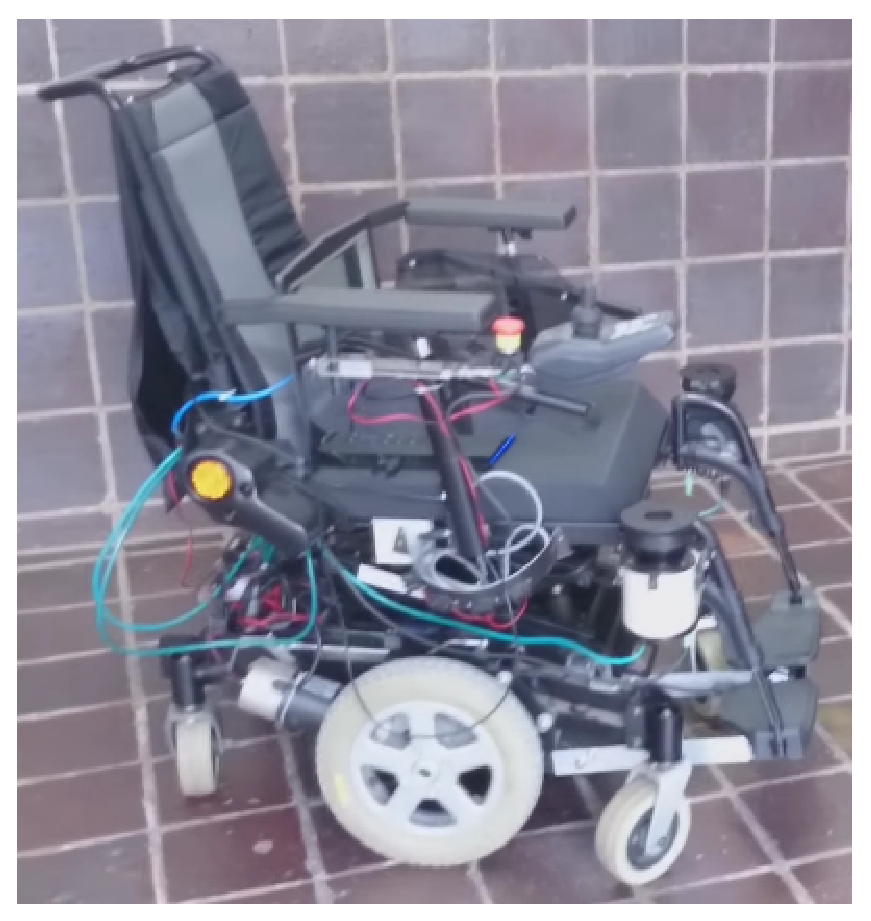
\includegraphics[width=0.48\textwidth]{images/cap3/Perenquen.eps}
  \end{center}
  \vspace{-20pt}
  \caption{Perenquén}
  \vspace{-10pt}
  \label{fig:Perenquen}
\end{wrapfigure}

El objetivo principal de este proyecto es el desplazamiento autónomo de una
silla de ruedas, mediante la detección de obstáculos de un entorno, así como su
localización en el mismo a través de las imágenes capturadas mediante la versión
2.0 de Kinect A diferencia de Verdino, Perenquén intenta ser una alternativa de
bajo coste frente a los sistemas de detección de obstáculo de Verdino.

Actualmente la silla cuenta con el dispositivo Kinect, un sistema de odometría
mecánica, y tres detectores láser (lado izquierdo, lado derecho y posterior) que
hacen posible una detección más precisa de los obstáculos.

%+++++++++++++++++++++++++++++++++++++++++++++++++++++++++++++++++++++++++++++++
